% =====================================================================
% DRAFT MODE: toggle this line to show or hide drafting aids.
\newif\ifdraft
\drafttrue % uncomment this line to toggle on the planning box, notes, and to-dos
%\draftfalse % uncomment this line to hide notes, for sharing or submission
% =====================================================================

\documentclass[11pt]{article}

\usepackage[margin=1in]{geometry}
\usepackage[T1]{fontenc}
\usepackage{graphicx}
\usepackage{amsmath}         % better math
\usepackage{booktabs}        % nicer looking tables
\usepackage[round]{natbib}   % author-year citations with \citet and \citep
\usepackage{xcolor}
\usepackage{tcolorbox}       % box for the planning notes
\usepackage[hidelinks]{hyperref}

% Look for graphics in the figures folder, so \includegraphics needs only
% the file name. The scripts in calculations/ write to this folder.
\graphicspath{{figures/}}

% ---------------------------------------------------------------------
% Drafting aids, controlled by the \drafttrue/\draftfalse toggle at the top
% of this file. Change the colors here if you like.
\definecolor{notecolor}{HTML}{A51C30}  % crimson, for notes to coauthors
\definecolor{todocolor}{HTML}{1F3A68}  % navy, for to-dos and planning

% Line numbers stay on in both modes, since journals usually want them
% at submission and they help coauthors and reviewers comment on the text.
\usepackage{lineno}
\linenumbers

\ifdraft
  \newcommand{\note}[1]{\textcolor{notecolor}{#1}}
  \newcommand{\todo}[1]{\textcolor{todocolor}{[#1]}}
\else
  \newcommand{\note}[1]{}
  \newcommand{\todo}[1]{}
\fi
% With coauthors, give each person their own command and color, e.g.,
% \newcommand{\authorANote}[1]{\textcolor{notecolor}{Author A: #1}}
% (LaTeX command names can contain letters only, not digits.)
% ---------------------------------------------------------------------

\title{Title that states your main finding}
\author{First Author and Second Author}
\date{\today}  % a date helps coauthors confirm they have the latest draft

\begin{document}
\maketitle

% Planning notes: decide these before writing any prose. They appear only
% in draft mode, so they stay visible to you and your coauthors.
\ifdraft
\begin{tcolorbox}[colback=todocolor!4, colframe=todocolor, coltext=todocolor,
  title=Plan (hidden when \texttt{\textbackslash draftfalse})]
\textbf{Topic.} One sentence describing what the paper is about.

\medskip
\textbf{Audience.} Who needs these results, and what do they already know?

\medskip
\textbf{Draft conclusions.}
\begin{enumerate}
  \item First main conclusion, stated as a specific claim.
  \item Second main conclusion.
  \item Third main conclusion, if there is one.
\end{enumerate}

\textbf{Target journal.} Journal name, and what its readers expect. Check its length limits and required sections.

\medskip
\textbf{Coauthors.} Who is contributing, and who else should be invited?
\end{tcolorbox}
\fi

\begin{abstract}
\todo{Draft the abstract after the outline and before the rest of the text. In a few sentences, state the problem, what you did, what you found, and why it matters. Revise it once the paper is written.}
\end{abstract}


\section{Introduction}

\todo{Sketch the gap and contribution now, and write the full introduction last. Establish why the topic matters, identify what is missing from prior work, and state how this paper fills the gap.}

Cite related work with \texttt{\textbackslash citep} to put the authors inside the parentheses \citep{swales_1990}, or with \texttt{\textbackslash citet} to name them in the sentence, as in \citet{gastel_2022}.

\note{Here is a note to a coauthor. Notes and to-dos disappear when you set \texttt{\textbackslash draftfalse} at the top of this file.}


\section{Methods}

\todo{Describe what you did in enough detail that a reader could reproduce it. List the key assumptions.}

Equations are part of the evidence, so add them during outlining. For example, a multi-line equation aligned at the equals sign, with the number suppressed on the first line:
\begin{align}
F_{M}(m) &= P(M \le m) \nonumber \\
         &= 1 - 10^{-b(m - m_{\min})}
\end{align}


\section{Results}

\todo{Papers revolve around their figures, so put each figure here as soon as you have it, even a rough version. Then write text that describes and interprets each one.}

Figure~\ref{fig:demand_capacity} shows a single-panel figure, and Figure~\ref{fig:fragility} shows a two-panel figure. Both are generated by scripts in the \texttt{calculations} folder, so rerunning \texttt{make\_all\_figures.py} updates them.

\begin{figure}[htb!]
\centering
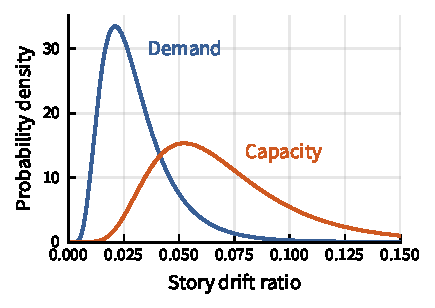
\includegraphics{demand_capacity}
\caption{Distributions of structural demand and capacity.}
\label{fig:demand_capacity}
\end{figure}

\begin{figure}[htb!]
\centering
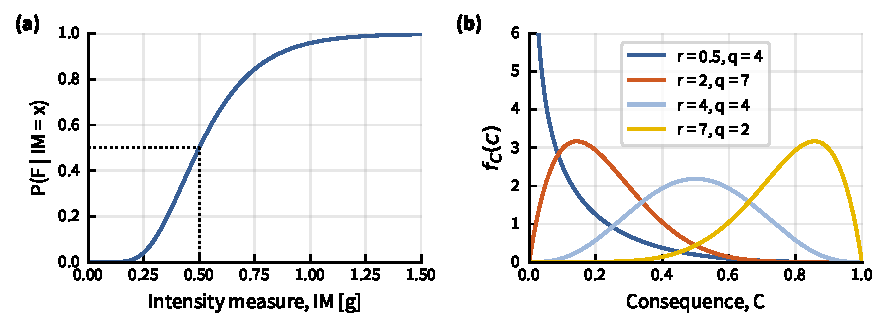
\includegraphics{fragility_and_consequences}
\caption{(a) Fragility function. (b) Consequence distributions for several parameter values.}
\label{fig:fragility}
\end{figure}

Table~\ref{tab:example} shows a simple table.

\begin{table}[htb!]
\centering
\caption{Table caption.}
\label{tab:example}
\begin{tabular}{lll}
\toprule
Case & Median & Dispersion \\ \midrule
Demand   & 0.027 & 0.50 \\
Capacity & 0.064 & 0.45 \\ \bottomrule
\end{tabular}
\end{table}


\section{Conclusions}

\todo{Restate the draft conclusions from the plan, now supported by the results above. Many readers skim this section first, so each conclusion should make sense on its own. Note limitations and what comes next.}


\bibliographystyle{plainnat}  % replace with your journal's .bst file
\bibliography{references}

\end{document}
